\chapter{\label{ch:via-ferrata-lacs-robert}Via Ferrata des Lacs Robert, Chamrousse}

\section*{The basics}

The \place{Via Ferrata des Lacs Robert} is an amazing mountain activity that takes a good part of the day and requires good lungs. Although it can be reached through \place{Croix de Chamrousse} mechanical ascent if it is open, here we will describe our adventure exactly as we have done it, walking all our way up there and back. Before engaging in this activity, consider checking the \emph{via} is open and meteorologic conditions are favorable to practice a \emph{via ferrata}. Under no circumstances do it under the rain! It is also important to contact the \href{https://www.chamrousse.com/plan-via-ferratas.html}{tourism office of \place{Chamrousse}} and check the \emph{vias} (actually there are two \emph{ferratas} up there, but here we stick to \place{Lacs Robert} only) are open before getting there.

\section*{Getting there}

We started the trekking at \place{Chamrousse 1650 - Le Recoin}, as displayed in Fig.~\ref{fig:map-ferrata-des-lacs-robert-start}. There is a parking if you intend to drive but it can also be reached by bus from \place{Grenoble}. As of 2022, in summertime line T87 leaving \place{Grenoble}'s train station deserves the location. Beware that on weekends there are only 3 trips a day and the first in the morning is required to be able to do the \emph{ferrata}. 

\begin{figure}[!h]
\centering%
\includegraphics[width=\columnwidth, clip]{media/maps/via-ferrata-des-lacs-robert-start}
\caption{\label{fig:map-ferrata-des-lacs-robert-start}Trekking starting point at Chamrousse 1650.}
\end{figure}

The trekking itself it mostly of average difficulty with a few parts being considered slightly difficult when approaching \place{Lacs Robert}. Walking sticks are recommended and at least 3 liters of water per person. One must also keep in mind that it starts at 1650~m above sea level and even during summer days temperatures could drop below 20$^\circ$C, so consider getting properly dressed. We did it on September 17th 2022, just 3 days before the end of summer, and the temperature was around 2$^\circ$C! Since the way up is to the west of the peaks you stay all the time on the shadow of the mountain and the sun will not heat you up. But don't worry, the altitude gain of about 400~m will do the job. Figure~\ref{fig:via-ferrata-des-lacs-robert-1} shows the magnificent view of the valley with \place{Saint-Nazaire-les-Eymes}.

\begin{figure}[!h]
\centering%
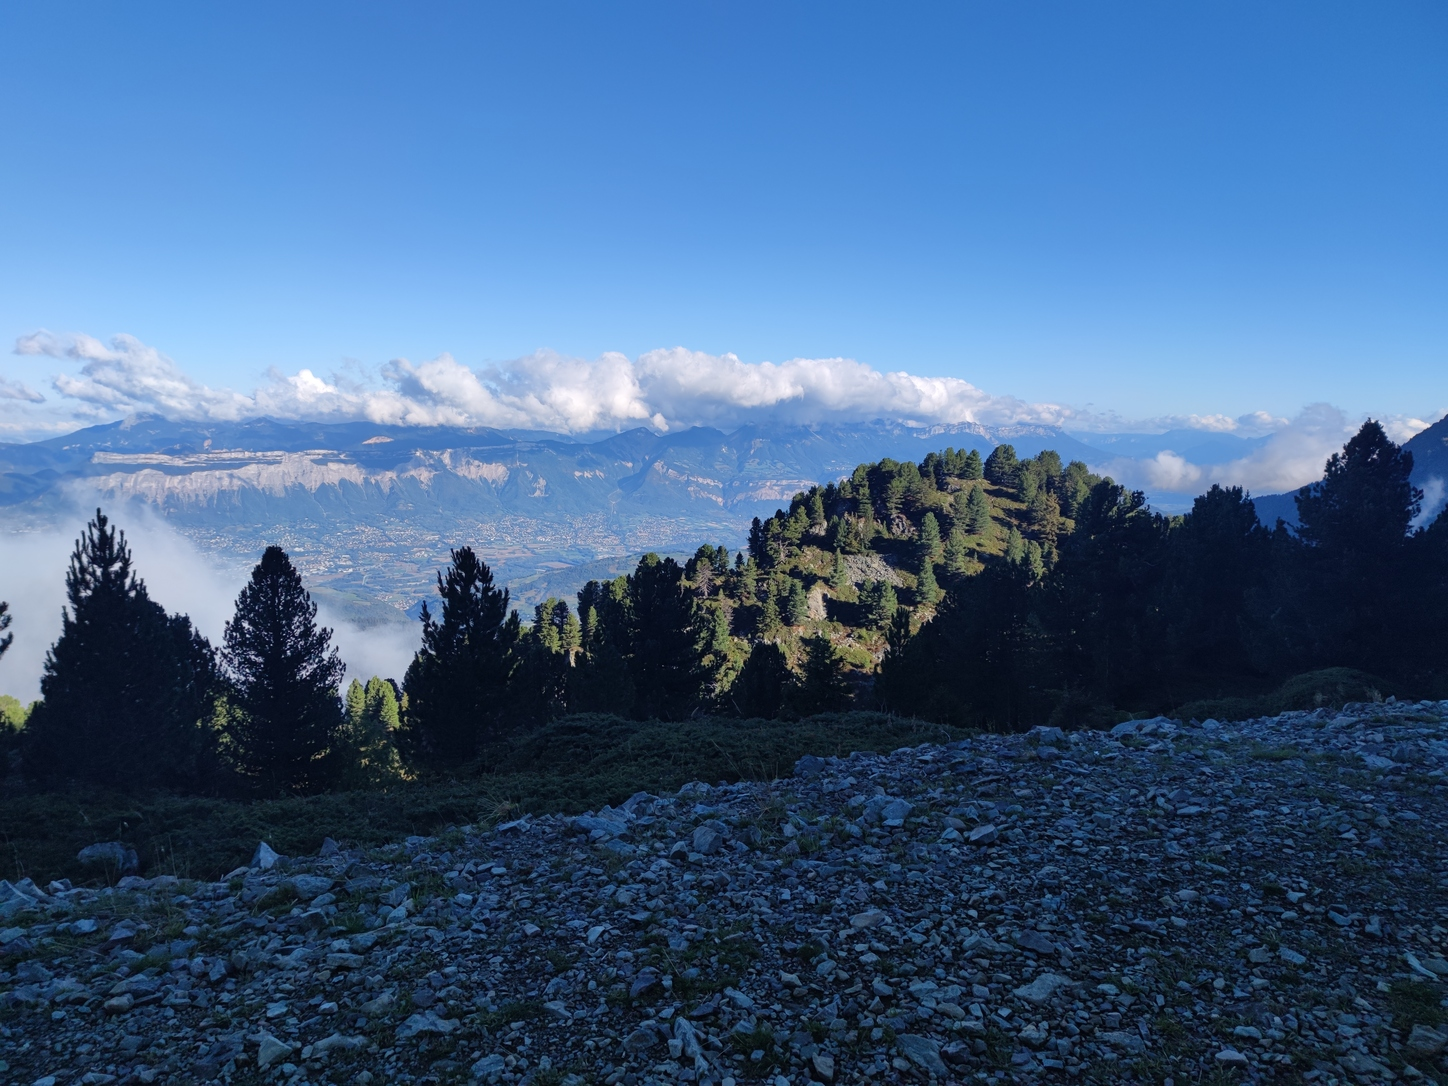
\includegraphics[width=\columnwidth, clip]{media/pictures/via-ferrata-des-lacs-robert-1}
\caption{\label{fig:via-ferrata-des-lacs-robert-1}View from about 2000~meters on the way up.}
\end{figure}

The first view of \place{Lacs Robert} in Fig.~\ref{fig:via-ferrata-des-lacs-robert-2} will tell that you have reached your destination. There are several nice spots to take shots there but I prefer to let you curious and go discover by yourself. You can go around the lake, it takes just a few minutes, and discover the mountain hut over there. The day we've been there the first time there were some people fishing and running around. It is better to make a short pause there and admire the nature before engaging in the \emph{ferrata}.
 
\begin{figure}[!h]
\centering%
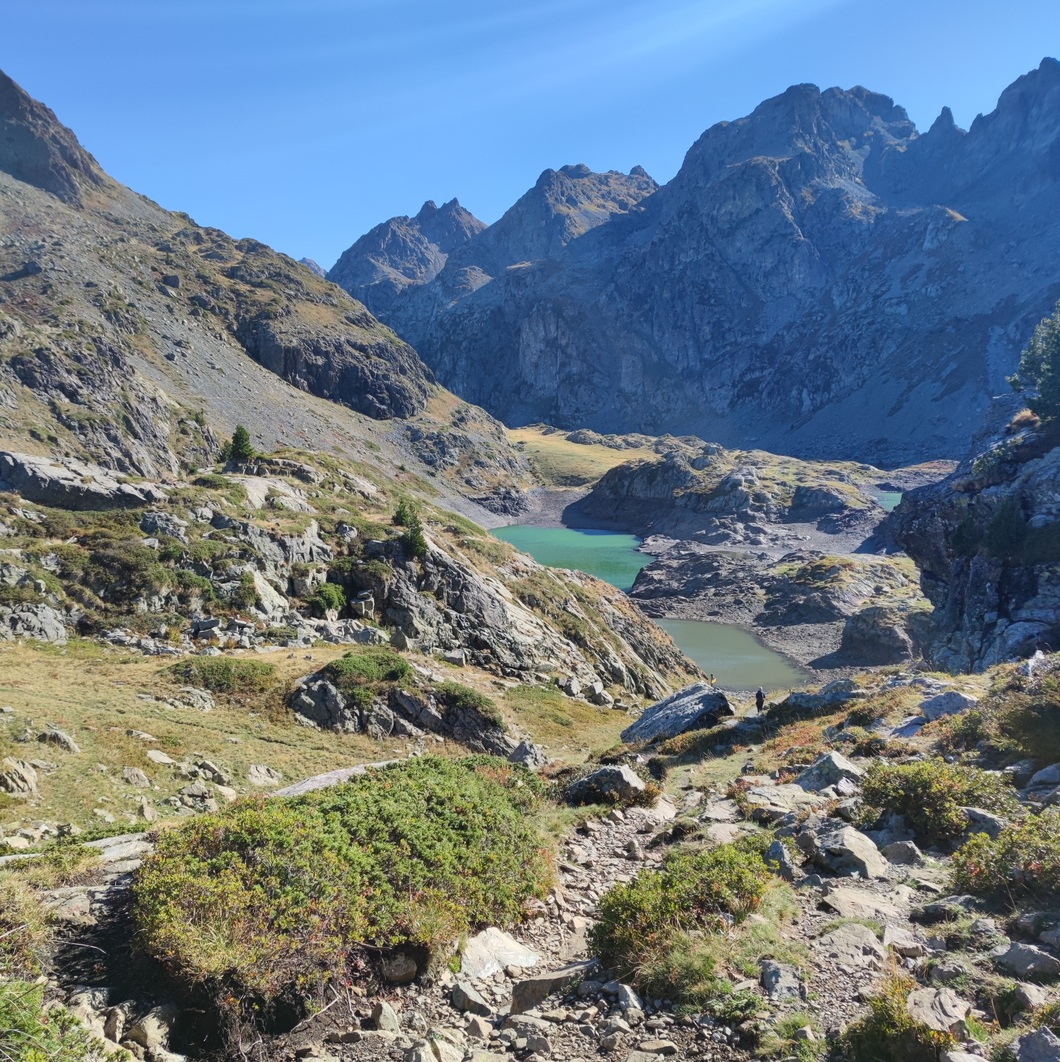
\includegraphics[width=\columnwidth, clip]{media/pictures/via-ferrata-des-lacs-robert-2}
\caption{\label{fig:via-ferrata-des-lacs-robert-2}Arriving at Lacs Robert.}
\end{figure}

Most of the guides I have found out there do not precisely state where to find the \emph{via}'s entry point. Assuming you are where the picture in Fig.~\ref{fig:via-ferrata-des-lacs-robert-2} was taken from, keep to the left and at the point opposed to the lake hut you can look up the hill to southwest direction and a panel indicating the start point will be there, as illustrated in Fig.~\ref{fig:map-via-ferrata-des-lacs-robert-entry}. There is no clear path to reach the starting point, so from here on it is some sort of savage trekking. Maybe consider wearing your \emph{ferrata}'s leather gloves and put your walking sticks in the bag because the vegetation is spiky and you could easily get a thorn in your hands.

\begin{figure}[!h]
\centering%
\includegraphics[width=\columnwidth, clip]{media/maps/via-ferrata-des-lacs-robert-entry}
\caption{\label{fig:map-via-ferrata-des-lacs-robert-entry}Via ferrata's starting point.}
\end{figure}

\section*{The via ferrata}

Once you have reached the aforementioned panel illustrated in Fig.~\ref{fig:via-ferrata-des-lacs-robert-3} it is time to gear-up. This via oriented towards east/southeast so in the morning it takes plenty of sun and temperatures are still fine for a comfortable climb. Consider a climbing time of 1h30 to 2h00 if you are experienced, a bit more if this is one of your first \emph{ferratas}. The total length of the \emph{via} is about 300~m and it goes from 2050~m to 2200~m, with a total level gain of 150~m. The way is difficult enough to difficult (French quotation AD/D), so beginners be aware your arms will get at least pretty tired.

\begin{figure}[!ht]
\centering%
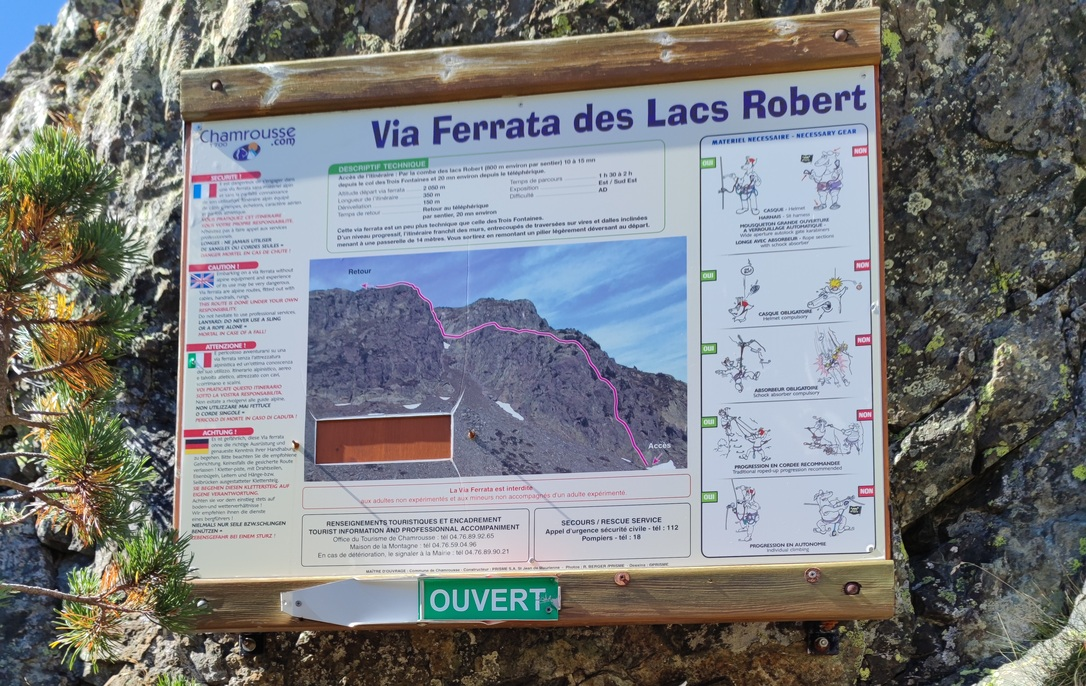
\includegraphics[width=\columnwidth, clip]{media/pictures/via-ferrata-des-lacs-robert-3}
\caption{\label{fig:via-ferrata-des-lacs-robert-3}Panel indicating the start of \emph{via ferrata}.}
\end{figure}

Since the via does not contain any zip line, a pulley is not required. The only special transversal in this \emph{ferrata} is a suspended bridge. Gear must include the basics, \begin{inparaenum}[(i)] \item a climbing harness, \item a climbing helmet, \item via ferrata gloves, and, most important and specific of all, \item energy-absorbing lanyards with two carabiners attached\end{inparaenum}. These days most of energy-absorbing lanyards are supplied already with \emph{via ferrata} specific carabiners. If yours is not, please notice that carabiners type K are mandatory for the practice of \emph{via ferrata}.

Also notice it is pretty vertical, so it is recommended that the most experienced person must be the first to climb and belay the others using climbing relay safety practices. That adds the typical sport climbing gear to the list, what includes \begin{inparaenum}[(i)] \item a belay device, \item a carabiner type H, and \item a rope, in this case about 30~m long should be enough\end{inparaenum}. If this is your first time doing a \emph{via ferrata}, consider getting professional support with a local guide. Since any mountain activity is considered high risk, do not forget a first aid kit, a cellphone, and portable batteries.

\section*{Getting back}

Once the \emph{via} is over you will be at 2200~m above sea level. A 15-minute-walk will lead you to \place{Croix de Chamrousse} (2253~m) from where you can chose to use the mechanical descent, if available, or engage in the trekking of \place{Crêtes} direction \place{Chamrousse 1850}. Notice that if you parked at \place{Chamrousse 1650} there is still another 40-minute-walk or wait for the last shuttle, what is recommended because some parts of the road are not deserved with a sidewalk, unless you want to try some more trekking.  The path is illustrated in Fig.~\ref{fig:map-via-ferrata-des-lacs-robert}, and can also be retrieved in my \href{https://www.alltrails.com/fr/explore/map/carte-29-decembre-2022-af0a59d}{All Trails} profile.

\begin{figure}[!h]
\centering%
\includegraphics[width=\columnwidth, clip]{media/maps/via-ferrata-des-lacs-robert-loop}
\caption{\label{fig:map-via-ferrata-des-lacs-robert}Path to reach Lacs Robert starting from Chamrousse 1650  (red), and to get back to Chamrousse 1850  (green).}
\end{figure}

\endinput